% =============================================================================
\section{Object Decomposition}
\label{sec:objects}
% =============================================================================

\subsection{Detection, Typing and Verification}

Objects are segmented on the original panorama with
SAM~2~\cite{ravi2024sam2segmentimages}, tiled and merged to handle equirectangular
distortion. Each crop is classified by CLIP against a fixed category set, with a
BLIP caption~\cite{li2022blipbootstrappinglanguageimagepretraining} as fallback
where the image pass is indeterminate. Labels are then verified by asking
Grounding DINO~\cite{liu2024groundingdino} to localize the proposed label in the crop:
CLIP proposes, an independent model disposes.

The reason for verification is that CLIP scores a fixed label set and always
returns a ranking, so even where it has no real signal some label still wins. The
ranking alone cannot distinguish a confident match from a near-uniform one, which
is why the decision is referred to a model that has to find the label in the
image rather than merely rank it.

\subsection{Correlation and Clustering}

Surviving detections are grouped by class, then sub-clustered by visual similarity
using DINOv2 embeddings and agglomerative clustering, splitting a class into
appearance variants (flower colors, tree species). Bucket counts are bounded, and
undersized buckets folded into their nearest neighbor, because an unbounded
distance cut produces one bucket per instance, measured at 302 groups on one
capture, each demanding its own reconstruction.

\begin{figure}[htbp]
  \centering
  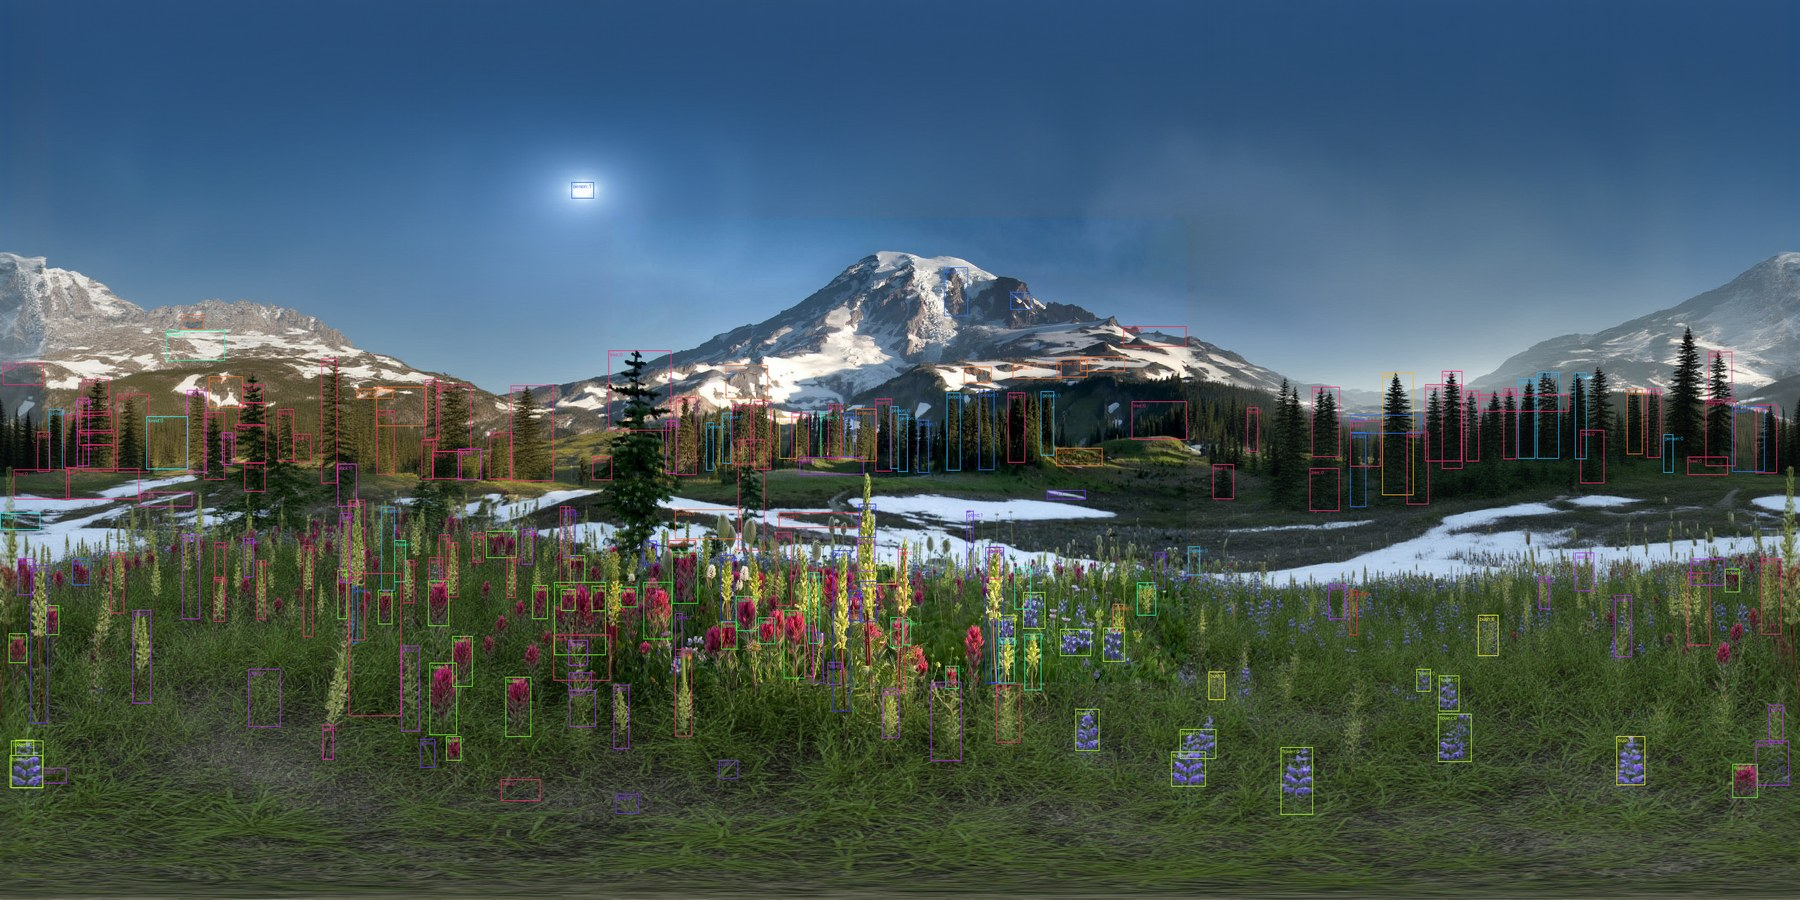
\includegraphics[width=\linewidth]{rainier/clusters.jpg}
  \caption{Detections on the Rainier panorama after appearance clustering, drawn in
  panorama pixel space and colored by bucket. Segmentation runs on the original
  panorama rather than the hero photograph, so detections cover the full
  $360^\circ$. Distinct buckets separate the conifers on the skyline from the
  flowering plants underfoot, and split the flowers themselves by color; each
  surviving bucket costs one reconstruction. The density in the near-field meadow is
  what motivates the population synthesis of \cref{sec:distribution} rather than
  per-instance reconstruction.}
  \label{fig:rainier-clusters}
\end{figure}

\subsection{Asset Generation and Level of Detail}

One mesh is reconstructed per (class, bucket) group with
SAM~3D~\cite{sam3dteam2025sam3d3dfyimages} and instanced at every member's
position. Two selection decisions matter.

The crop fed to reconstruction is chosen by \emph{resolution} among those passing
quality gates, not by classifier score, because a single-view reconstructor given too few pixels does not return a worse
object but a different one: a flat sheet. And the representation decision is made
on \emph{projected angular size} rather than distance, since distance only proxies
resolvability when every object is the same size.

That second decision picks one of three representations, in order of preference.
An instance is placed as a reconstructed \emph{mesh} when its group has one and it
renders large enough to resolve as geometry. Failing that it takes a \emph{crossed
card}: three fixed planes carrying the group's own photograph, twelve triangles
that hold their silhouette from any angle. A \emph{billboard}, a single quad that
rotates to face the viewer, is the last resort. Keeping the cheap tiers is what
makes the geometry budget hold without deciding resolvability by a proxy.

Cards are published only for vegetation, because vegetation is where both other
options fail. Single-view reconstruction of a conifer returns a sheet, under a
tenth as thick as it is wide on the Rainier capture, which the shape gates
correctly reject; and in stereo at the distance trees actually stand, a
camera-facing quad reads as flat and swings as the head moves. A rejected
reconstruction therefore falls back to a card rather than a billboard whenever its
class has one, which is why the same rejection yields cards for Rainier's trees and
billboards for Shark Fin's rock fragments (\cref{tab:results}). Because a card is
an ordinary textured mesh, it also inherits the sway rig of \cref{sec:lighting}
instead of standing still beside animated neighbors.

\subsection{World-Space Placement}
\label{sec:placement}

Detection, typing and reconstruction all operate in panorama pixel space or on an
isolated crop; nothing so far has produced a world position. Scene Assembly closes
that gap for every instance, real detection or synthesized fill alike, through the
same path: unproject the box into a metric position and extent, correct that extent
against the scene's own measured compression, snap its base to whichever ground
surface actually sits beneath it, and resolve collisions against everything already
placed.

\paragraph{Unprojection.} A box is unprojected using the panoramic depth measured at
stage 5 (\cref{tab:stagemodels}), before foreground removal, not the depth
recomputed at stage 16 on the object-removed panorama, which has since had the
region under every real object replaced by reconstructed background and would
silently misplace exactly the objects most likely to have just been removed. Extent
is measured as a vertical segment on the plane tangent to the object's own
horizontal distance $r$, not as the chord between the box's top and bottom edges on
the depth sphere: the chord $2r\sin(\Delta\phi/2)$ tracks true angular extent only
while $\Delta\phi$ is small and is bounded by $2r$ regardless of how tall the object
is, so it understates a tall, near object worst where it is most visible, and a
10 m tree at 4 m measured 5.92 m against 8.14 m at 8 m -- visibly smaller the closer
it stood. The tangent form,
\begin{equation}
  \text{height} = r\,\big(\tan\phi_{\text{top}} - \tan\phi_{\text{bottom}}\big),
\end{equation}
is exact at every distance and matches what the perspective-image path already
computes by construction. Because $\tan$ is convex, the box's vertical midpoint on
that same plane is not the point the center ray passes through either, so the
object is centered on the plane's midpoint rather than the ray, or a corrected
height ends up attached to the wrong center and the instance no longer subtends the
angle its own crop does.

\paragraph{Metric correction.} World size is computed as angular extent times
depth, so it inherits every depth-map compression at full strength
(\cref{sec:panorama}): the far-range compression that keeps distant terrain inside
the grid budget also miniaturizes anything standing on it, and because object size
is not measured independently anywhere else in the pipeline, nothing downstream can
tell the difference between a small object and a distant one rendered small.
Recovering scale therefore has to come from semantics rather than geometry. Classes
with a tight real-world height prior -- person \SI{1.70}{\meter}, car
\SI{1.50}{\meter}, and a dozen others weighted by how tightly the class actually
constrains height -- each yield one estimate of how far scale has drifted at that
instance's depth, pooled across the scene, binned by depth, and fit into a
monotonic depth$\to$correction curve, clamped and never extrapolated past the
fitted range: extrapolating would fabricate the largest correction exactly where
evidence is thinnest, for the far objects a truncated box is also most likely to
misreport. The curve is applied to every instance's size, never its position, which
stays exactly where the depth map put it and still snaps to the same terrain point.
A capture with no anchor class -- a wilderness scene with no person, car or bench
anywhere -- returns no fit at all, which leaves every object the size its own
measurement implies rather than guessing.

\paragraph{Ground snapping.} Object positions carry the full extrinsics
translation, while the terrain, water and formation meshes are all authored with
the camera at their local origin, so an object's world $(x, z)$ has to be
translated and un-rotated back into that native frame before it means anything to
the terrain. A downward raycast against every ground-capable mesh then resolves the
object's base height, taking the \emph{highest} surface at that point: the base
terrain is deliberately depressed under a rock formation and carved half a meter
below the water surface it carries, so raycasting the base terrain alone would bury
anything standing on a formation or at a shoreline by the depression depth plus the
object's own height. Where the raycast misses -- near the finite terrain grid's
edge, most often -- a dense height-map grid the terrain mesh was itself built from
serves as a fallback, so a missed snap degrades to the same reconstructed elevation
rather than to the object's own unprojected $y$, which was never reconciled with
the terrain and is what previously rendered as objects floating above, or sunk
into, the ground.

\paragraph{Deconfliction.} Every instance claims a circular footprint at its final,
snapped position, tested only against instances whose vertical extent actually
overlaps it, so an object standing atop another is never mistaken for one
intersecting it. Real detections claim ground before the synthesized fill of
\cref{sec:distribution}, ordered within each group by descending detector score, so
a measured object is never displaced by decoration and a weak duplicate detection
yields to a strong one rather than to whichever was enumerated first.
